\subsection{Snapshot Deduplication and Fault Isolation}
\label{sect:dedupe}
%snapshot representation


\subsection{Inner and corss VM deduplication}

Our  deduplication scheme compares the fingerprints of the current snapshot
with its parent snapshot and also other snapshots in the entire cloud.
This process performs   the duplication in two categories: \textit{Inner-VM} and \textit{Cross-VM}. 
Inner-VM duplication exists between VM's snapshots, because the majority of data are unchanged during each backup period. 
Such localization increases data independency between different VM backups,
simplifies snapshot management and statistics collection,
and facilitates parallel execution of snapshot operations.
On the other hand, Cross-VM duplication is mainly due to widely-used software and libraries. 
As the result, different VMs tend to backup large amount of highly similar data.
Our multi-level pipeline process can minimize 
the cost of deduplication while maximize the its efficiency at each level,
and it is parallel since each segment is processed independently.

\begin{itemize}
\item \textbf{Dirty-based corase-grain inner-VM deduplication.}
The first-level deduplication is to follow the standand dirty bit approach, but is conducted
in the coarse grain segment level.
We use the  Xen virtual device driver which supports dirty bits for thestorage device
and the dirty bit setting is maintained in a corase grain level we call it a segment.
In our implementation, the segment size is 2MB. 
Since every write for a block will touch a dirty bit, the device driver maintains dirtybits in memory
and cannot affort a small segment  size.

\item \textbf{Chunk-level fine-grain nearby duplicate detection.}

The best deduplication uses a nonuniform chunk size 
in the average of 4K or 8K~\cite{??}.
Thus the second-level inner-VM deduplication is to assess in this
level, but only for those dirty  segments. 
We load the fingerprints of block chunks of the corresponding segment from the
parent for a comparisons and compare near-by fingerprint matching within this segement.
The amount of memory for maintaining those fingerprints  is small.
For example, with a 2MB segment, there are about 500 fingerprints to compare.


%If we use 4KB in level-1, then such a level-1 should have similar dedup efficiency 
%as the current level-1 and level-2 combined, because finally they equal to comparing  
%parent snapshot at 4KB granularity.
%
%However, at level-3 things are different. If we use 4KB fix-size block uniformly, it would be harder for different VM to share data through CDS, because there is no guarantee that the location of duplicate data on different VM disks are always aligned at 4KB boundary. For example, if two VMs each has a copy of duplicate data, but they are not aligned, then we won't be able to detect them. Our study at the current small data set has shown that using 4KB fix-size block will make CDS method less efficient by nearly 10%. Over the long time, more and more OS variations will co-exist in the cluster, making this 4KB fix-size approach inefficient in reducing duplicate data across VMs.

%\item \textit{Level 2  Chunk fingerprint comparison.}
%If a segment is modified, we perform fine-grained deduplication 
%by comparing the fingerprints of its chunks to the same segment's recipe in the previous snapshot,
%thus eliminate partial data duplication within the segment.
%\end{itemize}
%
%In general, operations at level 1 have almost no cost and most of unmodified data are filtered here. 
%To process a dirty segment at level 2, 
%there requires no more than one DFS access to load the segment recipe from previous snapshot,
%and a tiny amount of memory to hold it in main memory.

\item \textbf{Cross-VM deduplication.}
This step accomplishes the standand global fingerprint  comparison as conducted
in the previous work~\cite{??}.
One key observation is that the inner deduplication has removed many of duplicates.
There are not lot of deduplication opportunities cross VMs while the memory
consumption for global comparison is expensive.
Thus our approximation is that duplicate sharing patterns among  VM follows
a zip-like distribution, and the global fingerprint  comparison  only searches
for the most popular items. 
\end{itemize}

\subsection{Popular Chunk Management and VM-oriented Fault Isolation}


Our objective for fault isolation is to minimize the number of VMs affected when there are failures
in the cluster.  The inner-VM deduplication does not depend on any global service and the comparison
for each VM is localized within the parent and the current snapshot.
Thus there is no data dependence between VMs.
For cross-VM deduplication, there is a data dependence among VMs and we would minimize the faiulre impact
of shared blocks by adding extra replcas of those shared blocks.

 

 
{\bf Snapshot Representation}.
The virtual device driver uses a bitmap to track the changes 
that have been made to virtual disk.
Every bit in the bitmap represents a fix-sized (2MB) region called \textit{segment}, indicates whether the segment
is modified since last backup. Hence we could treat segment as the basic unit in snapshot backup similar to
file in normal backup: a snapshot could share a segment with previous snapshot it is not changed. 
Moreover, we break 
segments into var-sized chunks (average 4KB) using content-based chunking algorithm,
which brings the opportunity of fine-grained deduplication by
allowing data sharing between segments.

\begin{figure}[htbp]
  \centering
  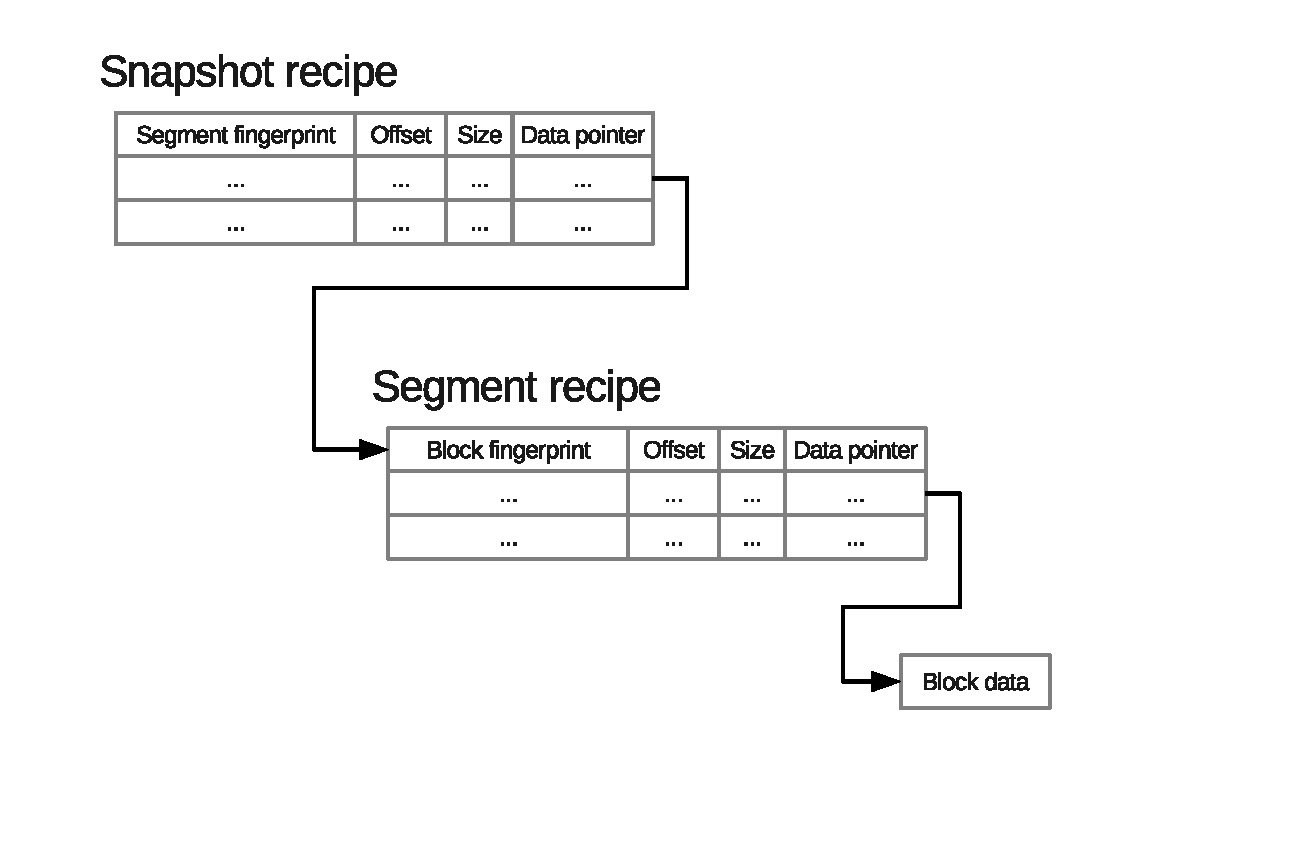
\epsfig{file=images/snapshot_representation.eps, width=3.7in}
  \caption{An example of snapshot representation.}
  \label{fig:snapshot}
\end{figure}
As a result, the representation of each snapshot is designed as a two-level index data structure 
in the form of a hierarchical directed acyclic graph as shown in Figure \ref{fig:snapshot}.
A snapshot recipe contains a list of segments, each of which is represented as a segment recipe
that holds the meatdata of its chunks. We choose this two-level structure because in practice we
observe that during each backup period only a small amount of VM data are added or modified. 
As the result, even the metadata of two snapshots can be highly similar, 
thus aggregating a large number of chunks as one segment can significantly reduce the space cost of snapshot metadata.
Furthermore, instead of using variables-sized segments, we use a dirty bit to capture the change status of fix-sized
segments which greatly ease the segment-level deduplication.

In both two kind of recipes, 
they do not include the actual data but only have
 references point to the data which are either stored in append store or CDS.
In our implementation the data reference is a 8 bytes field which is either an 
ASID (discuss in \ref{sect:append} or an offset of 
An additional flag indicates



